\documentclass[11pt,a4paper]{article}
\usepackage[utf8]{inputenc}
\usepackage{amsmath}
\usepackage{amsfonts}
\usepackage{amssymb}
\usepackage{graphicx}
\author{Dainius Jocas}
\title{In the Dalvik}
\begin{document}
\maketitle

The Dalvik Virtual Machine is the heart of Android. It's a fast, just-in-time compiled, optimized bytecode virtual machine. Android applications are compiled to Dalvik bytecode and run on the Dalvik VM. This section includes detailed information such as the Dalvik bytecode format specification, design information on the VM itself, and so on.

Dalvik is the managed runtime used by applications and some system services on Android. Dalvik was originally created specifically for the Android project.

Today we are going to start to look at the code which is at the very core of Dalvik VM (Virtual Machine). To be more specific, we are going to talk about Android's run-time system, whose core part is the Dalvik VM. 

By definition run-time system is a software designed to support the execution of computer programs. Intuitively, we can think of a runtime as a set of libraries that is responsible for low level tasks, e.g. dynamic memory allocation in C. In addition to the basic low-level tasks of the program, a runtime system may also implement higher-level behaviour and even support type checking, debugging, or code generation and optimization. Dalvik as a runtime, besides providing low-level libraries, implements lots of higher-level functionality, e.g. type checking.

To investigate implementation of Dalvik, means to investigate an implementation of the run-time system. And, therefore, to investigate the implementation of the run-time system means to investigate the implementation of a set of tools of the run-time system, e.g. dexopt -- a tool which verifies and optimizes all of the classes in the DEX file.

Dalvik project, at the source code level, is a rich set of tools:
\begin{itemize}
  \item dalvikvm --  program to support a command-line invocation of the Dalvik VM.
  \item dexdump -- this tool is intended to mimic "objdump". Objdump displays information about one or more object files.
  \item dexgen -- the dex code generator project. It provides API for creating dex classes in runtime which is needed e.g. for class mocking.
  \item dexlist -- tool that lists all methods in all concrete classes in one or more DEX files.
  \item dexopt -- a tool which verifies and optimizes all of the classes in the DEX file.
  \item dx -- Dalvik eXchange, the thing that takes in class files and reformulates them for consumption in the VM.
  \item libdex -- tool which is responsible for accessing .dex (Dalvik Executable Format) files.
  \item opcode-gen -- set of scripts for modification of opcodes.
  \item tools -- This tool runs a host build of dalvikvm in order to preoptimize dex files that will be run on a device.
  \begin{itemize}
    \item dexdeps -- DEX external dependency dump. This tool dumps a list of fields and methods that a DEX file uses but does not define.
    \item dmtracedump -- is a tool that gives you an alternate way of generating graphical call-stack diagrams from trace log files (instead of using Traceview).
    \item gdbjithelper -- kind of disassembler.
    \item hprof-conv -- tool to strip Android-specific records out of hprof data.
  \end{itemize}
  \item vm -- actual implementation of a VM:
  \begin{itemize}
    \item alloc -- Garbage-collecting memory allocator.
    \item analysis -- Dalvik bytecode structural verifier. 
    \item compiler --
    \item hprof -- Preparation and completion of hprof data generation. 
    \item interp -- Main interpreter entry point and support functions.
    \item jdwp -- Java Debug Wire Protocol support. Prints a list of available JDWP processes on a given device. 
    \item mterp -- the opcode interpreter
    \item static opcode check;
    \item ...
  \end{itemize}
\end{itemize}

%\section{Experiments}
%
%Here we'll see detailed description of what happens in Android run-time when new application is started. The representation of that process will look like a sequence of method calls.

%% There is a class called Application, which will be the root class for an application to be launched.
%% TODO: check class Application
%% TODO: how to follow the native code? because once things are getting interesting -- bam! native call
%% we are not considering all the app preparation work. We assume that everything is already done.
%%  both aspects of synchronization: enforcing exclusive access to an object's state and establishing happens-before relationships that are essential to visibility.										
%% http://roylee17.blogspot.it/2011/02/zygote-initialization-flow.html
%% http://benno.id.au/blog/?tag=android&start=10			
%% One key concept of Android execution is that it is based on callbacks. When something interesting to you happens, the Android system will call on of your callback methods.																																																																																		

%\subsection{Crash the Activity}
%I made an experiment, where the program crashed at the startup time. Actually it is the time when activity is being launched. But for the beginning it might be OK. 
%
%So, here is the stacktrace of the situation that caused crash of the application.
%\tiny\begin{verbatim}
%04-30 17:22:23.791: E/AndroidRuntime(679): FATAL EXCEPTION: main
%04-30 17:22:23.791: E/AndroidRuntime(679): java.lang.RuntimeException: Unable to start activity
%    ComponentInfo{com.example.test/com.example.test.MainActivity}: java.lang.NullPointerException
%04-30 17:22:23.791: E/AndroidRuntime(679): 	at android.app.ActivityThread.performLaunchActivity(ActivityThread.java:2663)
%04-30 17:22:23.791: E/AndroidRuntime(679): 	at android.app.ActivityThread.handleLaunchActivity(ActivityThread.java:2679)
%04-30 17:22:23.791: E/AndroidRuntime(679): 	at android.app.ActivityThread.access$2300(ActivityThread.java:125)
%04-30 17:22:23.791: E/AndroidRuntime(679): 	at android.app.ActivityThread$H.handleMessage(ActivityThread.java:2033)
%04-30 17:22:23.791: E/AndroidRuntime(679): 	at android.os.Handler.dispatchMessage(Handler.java:99)
%04-30 17:22:23.791: E/AndroidRuntime(679): 	at android.os.Looper.loop(Looper.java:123)
%04-30 17:22:23.791: E/AndroidRuntime(679): 	at android.app.ActivityThread.main(ActivityThread.java:4627)
%04-30 17:22:23.791: E/AndroidRuntime(679): 	at java.lang.reflect.Method.invokeNative(Native Method)
%04-30 17:22:23.791: E/AndroidRuntime(679): 	at java.lang.reflect.Method.invoke(Method.java:521)
%04-30 17:22:23.791: E/AndroidRuntime(679): 	at com.android.internal.os.ZygoteInit$MethodAndArgsCaller.run(ZygoteInit.java:868)
%04-30 17:22:23.791: E/AndroidRuntime(679): 	at com.android.internal.os.ZygoteInit.main(ZygoteInit.java:626)
%04-30 17:22:23.791: E/AndroidRuntime(679): 	at dalvik.system.NativeStart.main(Native Method)
%04-30 17:22:23.791: E/AndroidRuntime(679): Caused by: java.lang.NullPointerException
%04-30 17:22:23.791: E/AndroidRuntime(679): 	at com.example.test.MainActivity.onCreate(MainActivity.java:15)
%04-30 17:22:23.791: E/AndroidRuntime(679): 	at android.app.Instrumentation.callActivityOnCreate(Instrumentation.java:1047)
%04-30 17:22:23.791: E/AndroidRuntime(679): 	at android.app.ActivityThread.performLaunchActivity(ActivityThread.java:2627)
%04-30 17:22:23.791: E/AndroidRuntime(679): 	... 11 more
%\end{verbatim}
%\normalsize
%
%Let's see some important moments there:
%
%dalvik.system.NativeStart.main(Native Method)
%\begin{itemize}
%  \item /libcore/dalvik/src/main/java/dalvik/system/NativeStart.java
%  \item private static native void main(String[] dummy)
%  \item Dummy class used during JNI initialization.
%\end{itemize}
%
%com.android.internal.os.ZygoteInit.main(ZygoteInit.java:626)
%\begin{itemize}
%  \item ./frameworks/base/core/java/com/android/internal/os/ZygoteInit.java
%  \item Line 521
%  \item Startup class for the zygote process.
%\end{itemize}
%	
%java.lang.reflect.Method.invoke(Method.java:521)
%\begin{itemize}
%  \item ./libcore/luni/src/main/java/java/lang/reflect/Method.java
%  \item This class represents a method. Information about the method can be accessed, and the method can be invoked dynamically.
%\end{itemize}
%	
%java.lang.reflect.Method.invokeNative(Native Method)
%\begin{itemize}
%  \item private native Object invokeNative(Object obj, Object[] args, Class<?> declaringClass,
%            Class<?>[] parameterTypes, Class<?> returnType, int slot, boolean noAccessCheck)
%                    throws IllegalAccessException, IllegalArgumentException,
%                            InvocationTargetException;
%  \item 
%\end{itemize}
%
%android.app.ActivityThread.main(ActivityThread.java:4627):
%\begin{itemize}
%  \item ./frameworks/base/core/java/android/app/ActivityThread.java
%  \item 5017
%  \item This manages the execution of the main thread in an application process, scheduling and executing activities, broadcasts, and other operations on it as the activity manager requests.
%\end{itemize}
%	
%android.os.Looper.loop(Looper.java:123)
%\begin{itemize}
%  \item ./frameworks/base/core/java/android/os/Looper.java
%  \item Class used to run a message loop for a thread.
%\end{itemize}
%
%android.os.Handler.dispatchMessage(Handler.java:99):
%\begin{itemize}
%  \item ./frameworks/base/core/java/android/os/Handler.java
%\end{itemize}
%
%\subsection{Instrumentation}
%
%\begin{itemize}
%  \item ./frameworks/base/core/java/android/app/Instrumentation.java
%  \item onCreate(Bundle arguments) Called when the instrumentation is starting, before any application code has been loaded.
%  \item 
%\end{itemize}
%
%\subsection{Android Runtime}
%
%./frameworks/base/core/jni/AndroidRuntime.cpp
%
%Line 798: void AndroidRuntime::start Start the Android runtime.  This involves starting the virtual machine and calling the "static void main(String[] args)" method in the class named by "className".
%
%\subsection{app_main.cpp}
%
%Snippet from ./frameworks/base/cmds/app_process/app_main.cpp [Lines: 214:224]
%\tiny\begin{verbatim}
%    if (zygote) {
%        runtime.start("com.android.internal.os.ZygoteInit",
%                startSystemServer ? "start-system-server" : "");
%    } else if (className) {
%        // Remainder of args get passed to startup class main()
%        runtime.mClassName = className;
%        runtime.mArgC = argc - i;
%        runtime.mArgV = argv + i;
%        runtime.start("com.android.internal.os.RuntimeInit",
%                application ? "application" : "tool");
%\end{verbatim}\normalsize
%Here we see that there no big difference between startup of an Android system server and any other app -- just a branch of conditional statement.

\section{Second Experiment}

My task is to find the code which is executed in order to launch Android application. To do so I did an experiment.

The experiment is very trivial: I'm calling an activity which is not registered in the manifest file. This causes runtime crash, therefore, I can exploit stack trace to track the execution of the program. This simulates the overall execution of Android app because, this involves low level functionality, like finding code at runtime which needs to be executed.

To remaining part of the section would be organized in a following manner: first two subsection are the problem definition and the remaining part is a top-down approach of tracing the root cause of the runtime crash. Also, additional comments on the involved Android libraries will be provided.


\subsection{Who Calls onCreate()?}

Every activity that we are creating has a method with this notation:
\scriptsize\begin{verbatim}
@Override
protected void onCreate(Bundle savedInstanceState) {
    super.onCreate(savedInstanceState);
    setContentView(R.layout.activity_main);
    // place for your code
}
\end{verbatim} 
\normalsize
Who calls that method?

\subsection{Official documentation on the issue}

Figure from official Android documentation\footnote{http://developer.android.com/training/basics/activity-lifecycle/starting.html}:
\begin{figure}[ht]
  \center
  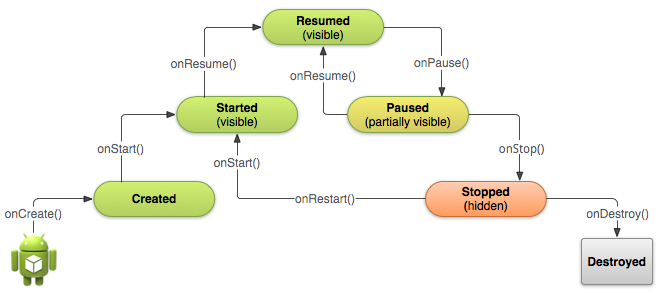
\includegraphics[width=\textwidth]{./images/basiclifecycle.png}
  \caption{Activity lifecycle.}
\end{figure} 


\subsection{Stack Trace}

Here I provide stack trace of the runtime error while execution call of an activity which does not exist.
\tiny
\begin{verbatim}
05-01 22:44:49.911: E/AndroidRuntime(1089): FATAL EXCEPTION: main
05-01 22:44:49.911: E/AndroidRuntime(1089): java.lang.RuntimeException: Unable to start activity ComponentInfo{com.example.test/com.example.test.MainActivity}: android.content.ActivityNotFoundException: Unable to find explicit activity class
 {com.example.test/com.example.test.DummyActivity}; have you declared this activity in your AndroidManifest.xml?
05-01 22:44:49.911: E/AndroidRuntime(1089): 	at android.app.ActivityThread.performLaunchActivity(ActivityThread.java:2663)
05-01 22:44:49.911: E/AndroidRuntime(1089): 	at android.app.ActivityThread.handleLaunchActivity(ActivityThread.java:2679)
05-01 22:44:49.911: E/AndroidRuntime(1089): 	at android.app.ActivityThread.access$2300(ActivityThread.java:125)
05-01 22:44:49.911: E/AndroidRuntime(1089): 	at android.app.ActivityThread$H.handleMessage(ActivityThread.java:2033)
05-01 22:44:49.911: E/AndroidRuntime(1089): 	at android.os.Handler.dispatchMessage(Handler.java:99)
05-01 22:44:49.911: E/AndroidRuntime(1089): 	at android.os.Looper.loop(Looper.java:123)
05-01 22:44:49.911: E/AndroidRuntime(1089): 	at android.app.ActivityThread.main(ActivityThread.java:4627)
05-01 22:44:49.911: E/AndroidRuntime(1089): 	at java.lang.reflect.Method.invokeNative(Native Method)
05-01 22:44:49.911: E/AndroidRuntime(1089): 	at java.lang.reflect.Method.invoke(Method.java:521)
05-01 22:44:49.911: E/AndroidRuntime(1089): 	at com.android.internal.os.ZygoteInit$MethodAndArgsCaller.run(ZygoteInit.java:868)
05-01 22:44:49.911: E/AndroidRuntime(1089): 	at com.android.internal.os.ZygoteInit.main(ZygoteInit.java:626)
05-01 22:44:49.911: E/AndroidRuntime(1089): 	at dalvik.system.NativeStart.main(Native Method)
\end{verbatim}
\normalsize

\subsection{class: Activity}

An activity is a single, focused thing that the user can do. Almost all activities interact with the user, so the Activity class takes care of creating a window for you in which you can place your UI with setContentView(View).

It's not that much surprising that the call is from the extended class:
\scriptsize\begin{verbatim}
final void performCreate(Bundle icicle) {
    onCreate(icicle);
    mVisibleFromClient = !mWindow.getWindowStyle().getBoolean(
            com.android.internal.R.styleable.Window_windowNoDisplay, false);
    mFragments.dispatchActivityCreated();
}
\end{verbatim}
\normalsize

File: ./frameworks/base/core/java/android/app/Activity.java

Line: 5108

Good start!

\subsection{class: Instrumentation}

Base class for implementing application instrumentation code.  When running with instrumentation turned on, this class will be instantiated for you before any of the application code, allowing you to monitor all of the interaction the system has with the application.

To executed code:
\scriptsize
\begin{verbatim}
/**
 * Perform calling of an activity's {@link Activity#onCreate}
 * method.  The default implementation simply calls through to that method.
 * 
 * @param activity The activity being created.
 * @param icicle The previously frozen state (or null) to pass through to
 *               onCreate().
 */
public void callActivityOnCreate(Activity activity, Bundle icicle) { 
    ...
    activity.performCreate(icicle);
    ...    
}
\end{verbatim}
\normalsize

File: ./frameworks/base/core/java/android/app/Instrumentation.java

Line: 1080

\subsection{class: ActivityThread}

This manages the execution of the main thread in an application process, scheduling and executing activities, broadcasts, and other operations on it as the activity manager requests.

\scriptsize
\begin{verbatim}
private Activity performLaunchActivity(ActivityClientRecord r, Intent customIntent) {
    ...
    mInstrumentation.callActivityOnCreate(activity, r.state); // line: 2144
    ...
}
private void handleLaunchActivity(ActivityClientRecord r, Intent customIntent) {
    ...
    Activity a = performLaunchActivity(r, customIntent); // line: 2230
    ...
}
\end{verbatim}
\normalsize

File: ./frameworks/base/core/java/android/app/ActivityThread.java 

Line: 2144

\scriptsize
\begin{verbatim}
public void handleMessage(Message msg) {
switch (msg.what) {
    case LAUNCH_ACTIVITY: {
        Trace.traceBegin(Trace.TRACE_TAG_ACTIVITY_MANAGER, "activityStart");
        ActivityClientRecord r = (ActivityClientRecord)msg.obj;

        r.packageInfo = getPackageInfoNoCheck(
                    r.activityInfo.applicationInfo, r.compatInfo);
        handleLaunchActivity(r, null); // line: 1234
        Trace.traceEnd(Trace.TRACE_TAG_ACTIVITY_MANAGER);
    } break;
    ...
}
\end{verbatim}
\normalsize


\subsection{class: Handler}

A Handler allows you to send and process Message and Runnable objects associated with a thread's MessageQueue. Each Handler instance is associated with a single thread and that thread's message queue. When you create a new Handler, it is bound to the thread / message queue of the thread that is creating it -- from that point on, it will deliver messages and runnables to that message queue and execute them as they come out of the message queue.

There are two main uses for a Handler: (1) to schedule messages and runnables to be executed as some point in the future; and (2) to enqueue an action to be performed on a different thread than your own. 

\scriptsize
\begin{verbatim}
    /**
     * Handle system messages here.
     */
    public void dispatchMessage(Message msg) {
        if (msg.callback != null) {
            handleCallback(msg);
        } else {
            if (mCallback != null) {
                if (mCallback.handleMessage(msg)) {
                    return;
                }
            }
            handleMessage(msg);
        }
    }
\end{verbatim}
\normalsize

Callback or not?

File: ./frameworks/base/core/java/android/os/Handler.java

Line: 90


\subsection{class: Looper}

Class used to run a message loop for a thread. Threads by default do not have a message loop associated with them; to create one, call prepare() in the thread that is to run the loop, and then loop() to have it process messages until the loop is stopped.

Most interaction with a message loop is through the Handler class. 

\scriptsize\begin{verbatim}
/**
 * Run the message queue in this thread. Be sure to call
 * {@link #quit()} to end the loop.
 */
public static void loop() {
   ...
   msg.target.dispatchMessage(msg);
   ...
}
\end{verbatim}
\normalsize

File: ./frameworks/base/core/java/android/app/ActivityThread.java

Line: 137


\subsection{class: ActivityThread}

Once again we are in this class, but it is because of the experiment.
\scriptsize
\begin{verbatim}
public static void main(String[] args) {
    ...
    Looper.loop(); // line: 5048
    ...
}
\end{verbatim}
\normalsize


\subsection{class Method}

This class represents a method. Information about the method can be accessed, and the method can be invoked dynamically. 

File: ./libcore/luni/src/main/java/java/lang/reflect/Method.java

\tiny
\begin{verbatim}
/**
 * This class represents a method. Information about the method can be accessed,
 * and the method can be invoked dynamically.
 */
...
public Object invoke(Object receiver, Object... args)
        throws IllegalAccessException, IllegalArgumentException, InvocationTargetException {
    if (args == null) {
        args = EmptyArray.OBJECT;
    }
    return invokeNative(receiver, args, declaringClass, parameterTypes, returnType, slot, flag);
}

private native Object invokeNative(Object obj, Object[] args, Class<?> declaringClass,
        Class<?>[] parameterTypes, Class<?> returnType, int slot, boolean noAccessCheck)
                throws IllegalAccessException, IllegalArgumentException,
                        InvocationTargetException; // line: 528
\end{verbatim}
\normalsize

So far, so good, but now the real mess begins.


\subsection{Native Method}

\scriptsize
\begin{verbatim}
File: ./dalvik/vm/native/java_lang_reflect_Method.cpp

/*
 * private Object invokeNative(Object obj, Object[] args, Class declaringClass,
 *   Class[] parameterTypes, Class returnType, int slot, boolean noAccessCheck)
 *
 * Invoke a static or virtual method via reflection.
 */
static void Dalvik_java_lang_reflect_Method_invokeNative(const u4* args,
    JValue* pResult)
{
\end{verbatim}
\normalsize

What happens here is that runtime didn't find a class to which the needed method belongs. 


\subsection{class: ZygoteInit}

Startup class for the zygote process.
 
Pre-initializes some classes, and then waits for commands on a UNIX domain socket. Based on these commands, forks off child processes that inherit the initial state of the VM.

\scriptsize
\begin{verbatim}
file: ./frameworks/base/core/java/com/android/internal/os/ZygoteInit.java
/**
 * Startup class for the zygote process.
 *
 * Pre-initializes some classes, and then waits for commands on a UNIX domain
 * socket. Based on these commands, forks off child processes that inherit
 * the initial state of the VM.
 ...
public static void main(String argv[]) {
    ...
    } catch (MethodAndArgsCaller caller) { //line 559
	...
	
\end{verbatim}
\normalsize


\subsection{Grey zone}

file: ./libcore/dalvik/src/main/java/dalvik/system/NativeStart.java
\scriptsize
\begin{verbatim}
/**
 * Dummy class used during JNI initialization.  The JNI functions want
 * to be able to create objects, and the VM needs to discard the references
 * when the function returns.  That gets a little weird when we're
 * calling JNI functions from the C main(), and there's no Java stack frame
 * to hitch the references onto.
 *
 * Rather than having some special-case code, we create this simple little
 * class and pretend that it called the C main().
 *
 * This also comes in handy when a native thread attaches itself with the
 * JNI AttachCurrentThread call.  If they attach the thread and start
 * creating objects, we need a fake frame to store stuff in.
 */
\end{verbatim}
dalvik.system.NativeStart.main(Native Method)

In other words: smoke and mirrors.

\subsection{Conclusion}

I have discovered how the Android framework deals with invoking new activity.

TODO:
Why looper? What is H class? JPEG in the latex.


\end{document}